%\documentclass[3p]{elsarticle}

% APS journals: PRL and PRF
% Note: All AIP and APS journals use the revtex package; both PRL and PRF are APS.
\documentclass[preprint, superscriptaddress, notitlepage]{revtex4-1}

%\documentclass{jfm}
% NOTE: jfm documentclass needed for \upi
%---------------------------------------------------%
% Packages from JFM 2020
%\usepackage[top=1.2in,bottom=1.2in,left=1in, right=1in]{geometry}
\usepackage{amsfonts, amssymb, array}
\usepackage[fleqn,reqno]{amsmath}
\usepackage{graphics, graphicx, subfigure}
% Replaced subcaption with subfigure
\usepackage{todonotes, comment, soul, float}
%---------------------------------------------------%

%^^^^^^^^^^^^^^^^^^^^^^^^^^^^^^^^^^^^^^^^^^^^^^^^^^^^^^^^^^^^%
% COMMANDS
% Basic editing
\newcommand{\tocite}{{\color{blue}(to cite)}}
\newcommand{\vsp}[1]{\vspace{#1 pc} \noindent}
\newcommand{\np}{\newpage \noindent}
% For real and imaginary, could use \Re or \Im, or \mathcal{R}, or \text{Re}
\newcommand{\Real}{\Re}
\newcommand{\Imag}{\Im}

%---------------------------------------------------%
% From JFM 2020
\newcommand{\bd}{{\partial}}
\newcommand{\bigO}{{\mathcal{O}}}
\newcommand{\cc}{{\mathbf{c}}}
\newcommand{\CC}{{\mathbb{C}}}
\newcommand{\DD}{{\mathcal{D}}}
\newcommand{\DDD}{{\boldsymbol{\mathcal D}}}
\newcommand{\eeta}{{\boldsymbol\eta}}
\newcommand{\ff}{{\mathbf{f}}}
\newcommand{\grad}{{\nabla}}
\newcommand{\II}{{\mathbf{I}}}
\newcommand{\iin}{\mathrm{in}}
\newcommand{\llambda}{{\boldsymbol\lambda}}
\newcommand{\nn}{{\mathbf{n}}}
\newcommand{\NN}{{\mathcal{N}}}
\newcommand{\out}{\mathrm{out}}
\newcommand{\rr}{{\mathbf{r}}}
\renewcommand{\Re}{{\operatorname{Re}}}
\renewcommand{\Im}{{\operatorname{Im}}}
\newcommand{\RR}{{\mathbb{R}}}
\renewcommand{\ss}{{\mathbf{s}}}
\newcommand{\ssigma}{{\boldsymbol\sigma}}
\newcommand{\tar}{\mathrm{tar}}
\newcommand{\bary}{\mathrm{bary}}
\newcommand{\trap}{\mathrm{trap}}
\newcommand{\uu}{{\mathbf{u}}}
\newcommand{\UU}{{\mathbf{U}}}
\newcommand{\vv}{{\mathbf{v}}}
\newcommand{\xx}{{\mathbf{x}}}
\newcommand{\xxi}{{\boldsymbol{\xi}}}
\newcommand{\yy}{{\mathbf{y}}}
\newcommand{\mcaption}[2]{\caption{\small \em #1}\label{#2}} 
\newcommand{\secref}[1]{\ref{#1}}
\def\gap{\hspace*{.2in}}
% Nick's below
\newcommand{\pderiv}[2]{\frac{\partial #1}{\partial #2}}
\newcommand{\ppd}[2]{\frac{\partial^2 #1}{{\partial #2}^2}}
\newcommand{\abs}[1]{\left| #1 \right|}
\newcommand{\Vn}{V_\nn}
\newcommand{\Vs}{V_\ss}
\newcommand{\CE}{C_E}
%---------------------------------------------------%



%^^^^^^^^^^^^^^^^^^^^^^^^^^^^^^^^^^^^^^^^^^^^^^^^^^^^^^^^^^^^%
% TITLE AUTHORS ABSTRACT
\begin{document}
\title{Fluid-mechanical erosion creates anisotropic porous media}
%\title{Fluid-mechanical erosion generates anisotropy in porous media}
%\title{Erosion leads to anisotropy in a porous medium}
%\title{The development of anisotropy in an eroding porous medium}


\author{Nicholas J.~Moore}
\affiliation{Department of Mathematics and Geophysical Fluid Dynamics Institute, Florida State University, Tallahassee, FL, 32306.}
\author{Bryan D.~Quaife}
\affiliation{Department of Scientific Computing and Geophysical Fluid Dynamics Institute, Florida State University, Tallahassee, FL, 32306.}
\author{Shang-Huan Chiu}
\affiliation{Department of Scientific Computing, Florida State University, Tallahassee, FL, 32306.}

\begin{abstract}
We numerically simulate the erosion of a porous medium due to an internally flowing fluid.  The solid constituents of the porous medium erode under the action of surface shear stress. As the particles disintegrate, they elongate in the direction of the flow, giving rise to anisotropic conductivity of the porous medium.
\end{abstract}
\maketitle
%^^^^^^^^^^^^^^^^^^^^^^^^^^^^^^^^^^^^^^^^^^^^^^^^^^^^^^^^^^^^%

%Shear stress on solid surfaces drives the erosion of porous material

% dematerialize, disintegrate

\section{Introduction}

Effects of flow-induced erosion are visible across a range of scales in nature, from massive geological structures, to mesoscopic patterns, and down to the tiny granular constituents that comprise a porous medium. In the case of a porous medium specifically, it has been long recognized that bulk properties of mediums encountered in nature are typically anisotropic, so that the medium allows flow in a preferred direction more easily. This anisotropy is commonly attributed to how grains are deposited, with their longest dimension parallel to the settling bed, so that they allow flow preferentially in the horizontal direction. Controlled experiments, however, have not been performed to test this hypothesis. Here, we use highly-accurate numerical simulations to examine an alternative, and possibly complementary, mechanism: namely, that the flow-induced erosion of the medium's solid constituents contributes to its overall anisotropy.

Our method merges highly-efficient and highly-accurate boundary-integral methods with stable interface evolution methods to simulate the erosion of many solid-bodies in the Stokes regime of groundwater flow \cite{Quaife2018}. Originally inspired by related work in the high-Reynolds-number regime \cite{Ristroph2012, Moore2013, Huang2015, MooreCPAM2017}, our method is documented, validated, benchmarked in \cite{Quaife2018}, and can simulate the erosion of order hundreds of solid bodies (please see \cite{Mitchell2016} for related work). The recent incorporation of barycentric interpolation methods permits simulation of tightly packed configurations (cite new paper with Shang). 

% Need to include descriptor 'high-fidelity' for our simulation.

Figure \ref{FigVortVel} shows an example illustration of 80 eroding bodies


%Maybe cite: \cite{Rycroft2016}
% Cite paper by Ladd "Wormhole formation in dissolving fractures"

%^^^^^^^^^^^^^^^^^^^^^^^^^^^^^^%
\begin{figure*}[] %\centering
        \subfigure[ Vorticity field]{ \label{FigVort}
            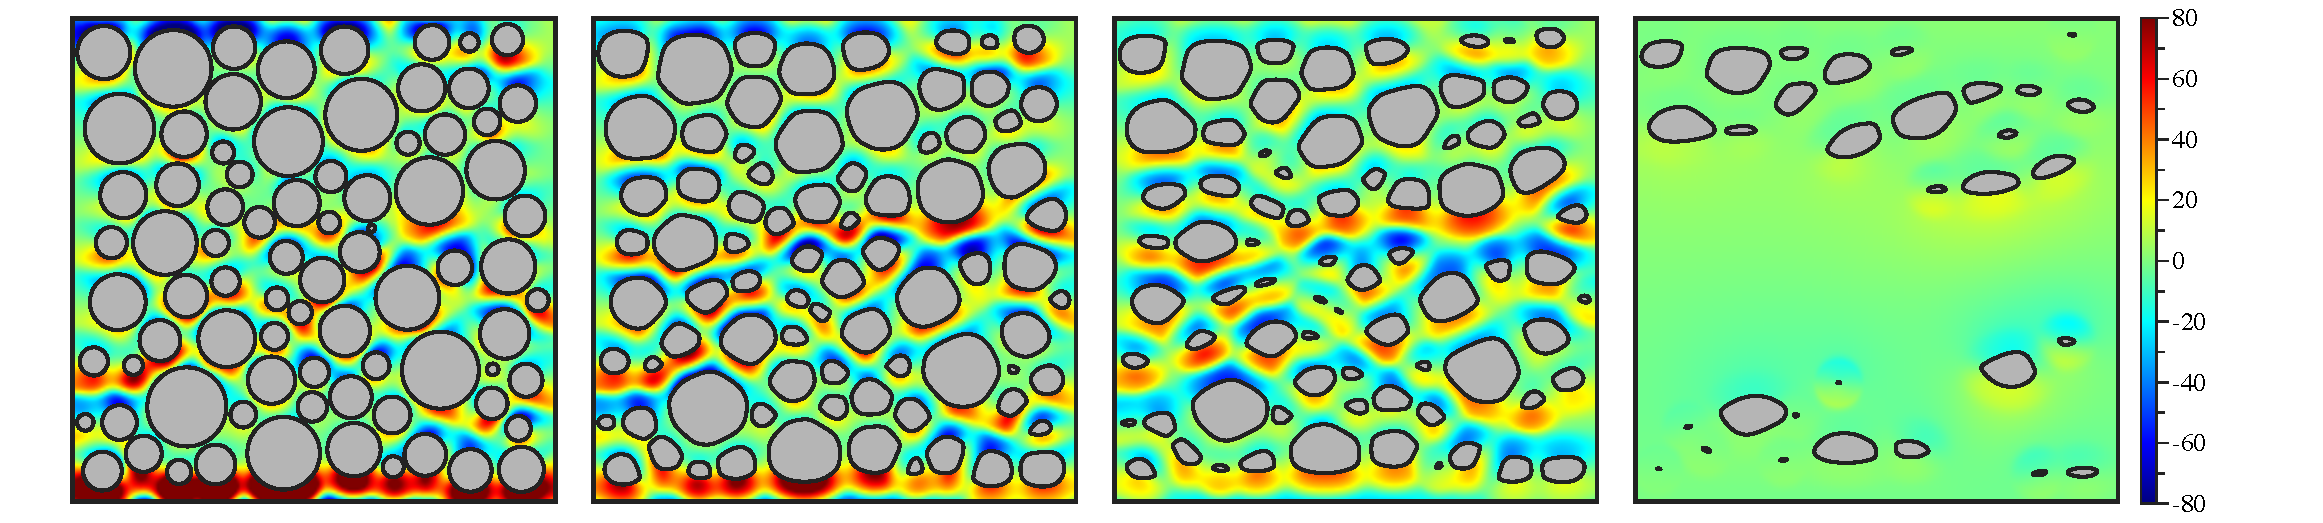
\includegraphics[width=0.9 \textwidth]{figs/80circ8vort.pdf} } \\
        \subfigure[ Velocity magnitude]{ \label{FigVel}
            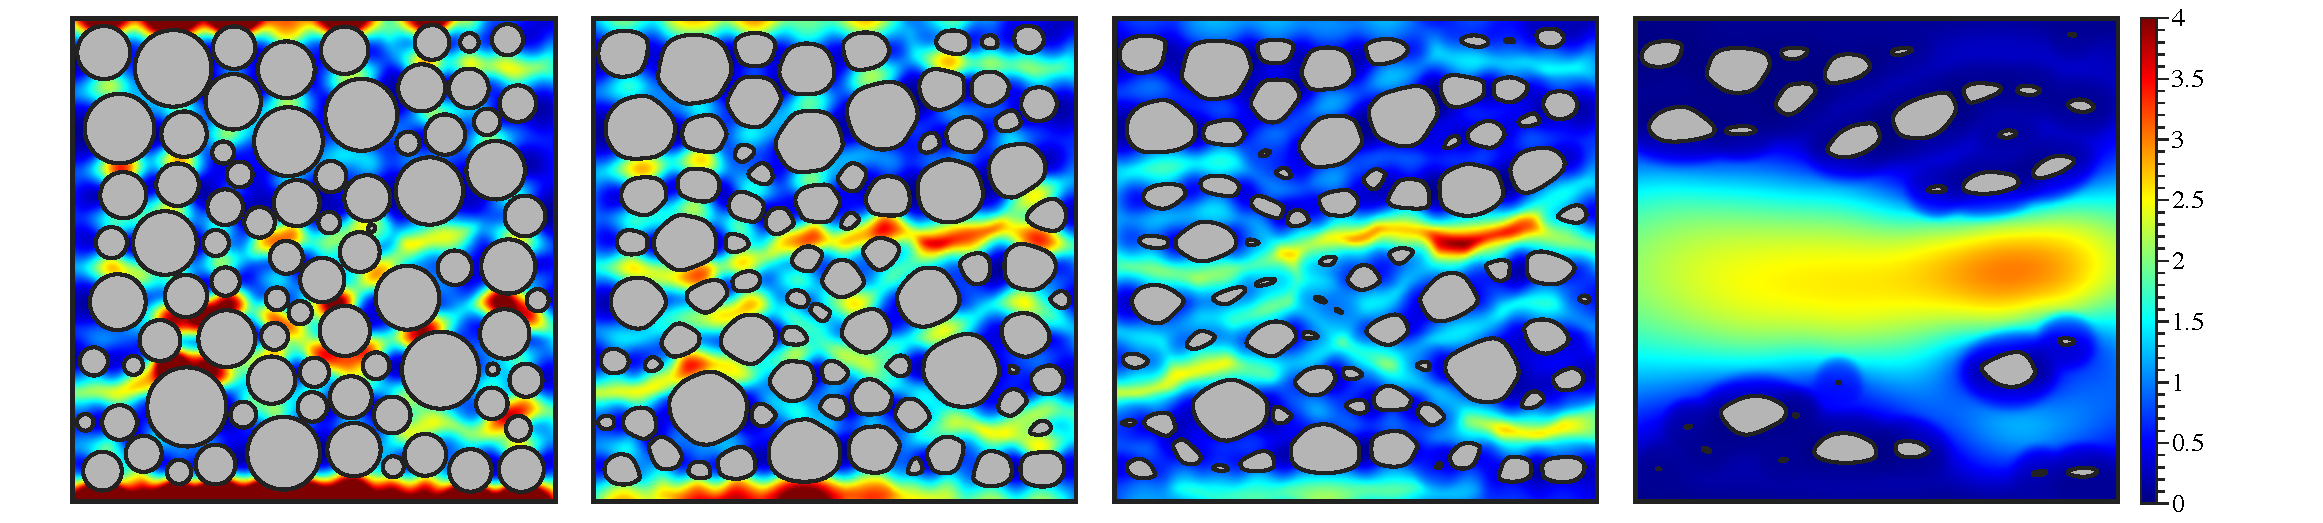
\includegraphics[width=0.9 \textwidth]{figs/80circ8vel.pdf} }
   \caption{80 eroding bodies}
   \label{FigVortVel}
\end{figure*}
%^^^^^^^^^^^^^^^^^^^^^^^^^^^^^^%
% Data from 80circ8



\begin{comment}
%^^^^^^^^^^^^^^^^^^^^^^^^^^^^^^%
\begin{figure*}%[htbp]
\centering \label{fig1}
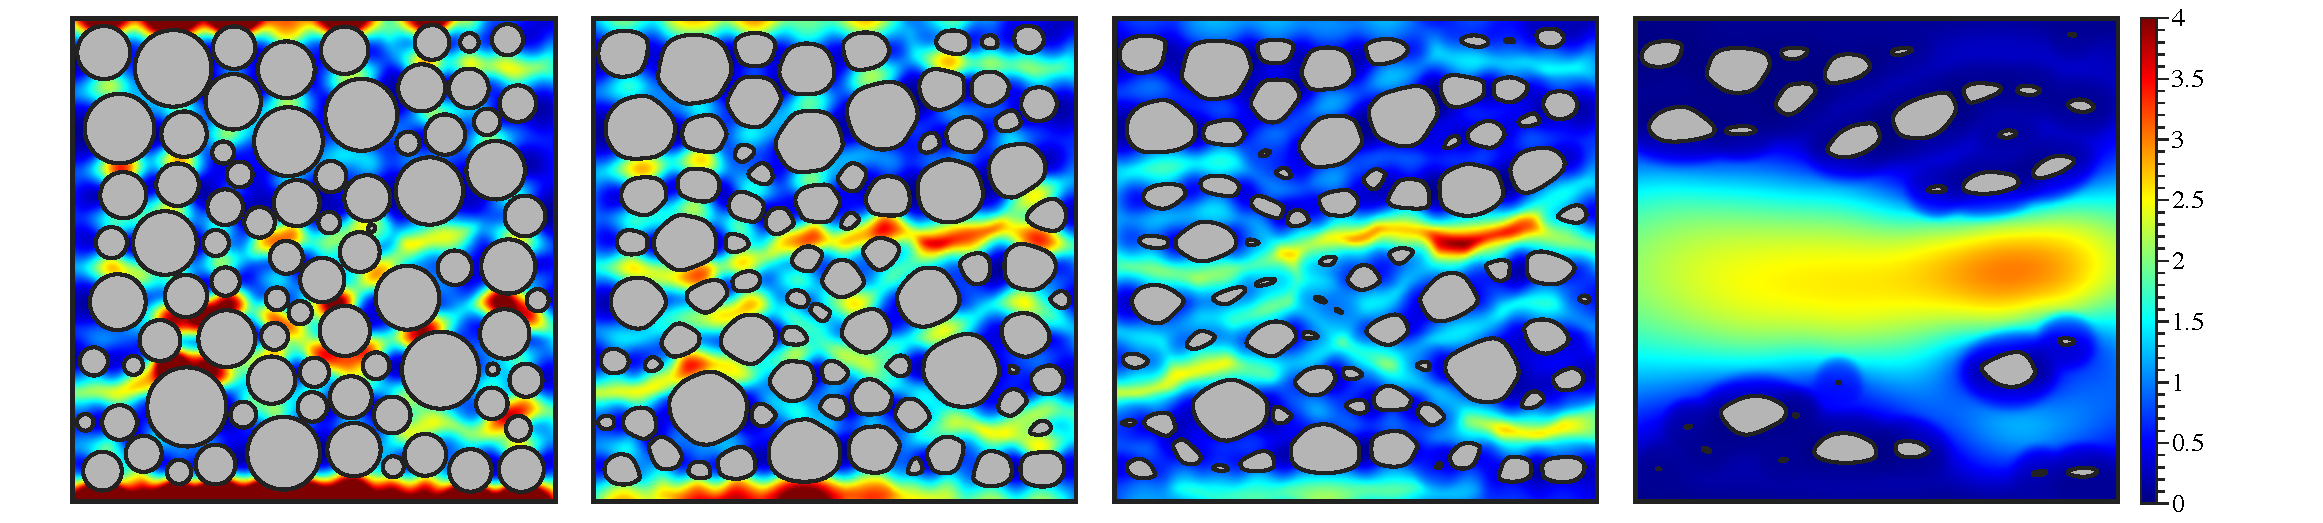
\includegraphics[width = 0.9 \textwidth]{./figs/80circ8vel.pdf}
\caption{caption}
\end{figure*}
 %^^^^^^^^^^^^^^^^^^^^^^^^^^^^^^%
\end{comment}



% NOTE: THIS SECTION HAS BEEN PLAGIARIZED FROM JFM 2020
% SO WE NEED TO PARAPHRASE IT
%\begin{comment}
%-----------------------------------------------------------------------------------------------%
\section{Governing Equations}
\label{sec:formulation}
%-----------------------------------------------------------------------------------------------%
We start by defining the main variables used to model erosion.  We only
briefly summarize the model, and a more detailed description can be
found in previous work~\citep{qua-moo2018}.  We consider flows inside a
confined geometry $\Omega$ that contains $M$ eroding bodies with
boundaries $\gamma_\ell$, $\ell = 1,\ldots,M$.  The boundary of the
fluid domain is $\bd \Omega = \Gamma \cup \gamma_1 \cup \cdots \cup
\gamma_M$, where $\Gamma$ is the outer boundary, taken to be a slightly
smoothed version of the boundary of $[-3,3] \times [-1,1]$.  All eroding
bodies are placed in $[-1,1] \times [-1,1]$ to create a buffer region
that allows the flow profile imposed at the inlet to transition to the
more complex flow intervening between the bodies. Neglecting inertial
forces, the governing equations are
\begin{equation}
\label{eqn:erosionModel}
  \begin{split}
    \mu \Delta \uu = \grad p, &\hspace{20pt} \xx \in \Omega, \gap 
      &&\mbox{\em conservation of momentum}, \\
    \grad \cdot \uu = 0, &\hspace{20pt} \xx \in \Omega, \gap 
      &&\mbox{\em conservation of mass}, \\
    \uu = \mathbf{0}, &\hspace{20pt} \xx \in \gamma, \gap 
      &&\mbox{\em no slip on the eroding bodies}, \\
    \uu = \UU, &\hspace{20pt} \xx \in \Gamma, \gap 
      &&\mbox{\em outer wall velocity}, \\
    \Vn = \CE \, \abs{\tau}, &\hspace{20pt} \xx \in \gamma,
      &&\mbox{\em erosion model}.
  \end{split}
\end{equation}
Here $\uu$ is the fluid velocity, $p$ is the pressure, $\UU$ is a
prescribed Hagen-Poiseuille velocity field, and $\Vn$ is the normal
velocity of $\gamma$. Since the rate of erosion is much slower than the
background flow, a quasi-steady approximation justifies the no-slip
boundary condition. Parameters include the fluid viscosity $\mu$ and the
material-dependent erosion constant $\CE$. By non-dimensionalizing
equations~\eqref{eqn:erosionModel}~\citep{qua-moo2018}, we set both
these parameters to one. The shear stress on $\gamma$ is
\begin{align}
  \tau = -(\nabla \uu + \nabla \uu^T) \nn \cdot \ss
  \label{eqn:shearStress}
\end{align}
where, $\nn$ is the normal vector pointing into the body, and $\ss$ is
the unit tangent vector pointing in the counterclockwise direction. We
simulate erosion by alternating between solving the fluid equations and
advancing the eroding grains.  The strength of $\UU$ is adjusted at each
time step to achieve a constant pressure drop across the channel,
motivated by the geological situation of a porous medium connecting two
regions of  fixed hydraulic heads.

%-----------------------------------------------------------------------------------------------%
\section{Boundary Integral Equation Formulation}
\label{sec:DLP}
%-----------------------------------------------------------------------------------------------%
To accurately solve the governing equations~\eqref{eqn:erosionModel} in
complex two-dimensional geometries, we reformulate the equations as a
BIE.  This has the advantage that only the one-dimensional boundary of
the domain must be discretized, and, with appropriate quadrature
formulas and fast summation methods, the result is a high-fidelity
numerical simulation with near-optimal computational complexity.

%-----------------------------------------------------------------------------------------------%
\subsection{Double-Layer Potential Formulation in $\RR^2$}
%-----------------------------------------------------------------------------------------------%
Applying the same approach as our previous work~\citep{qua-moo2018}, we
start with the double-layer potential 
\begin{align}
  \DDD[\eeta](\xx) = \int_{\bd\Omega} D(\xx,\yy) \eeta(\yy)\, ds_\yy = 
  \frac{1}{\pi}\int_{\bd\Omega} 
    \frac{\rr \cdot \nn}{\rho^2} \frac{\rr \otimes \rr}{\rho^2}
    \eeta(\yy) \, ds_\yy, \quad \xx \in \Omega,
  \label{eqn:velocityDLP}
\end{align}
where $D$ is the kernel of the integral operator, $\rr = \xx - \yy$,
$\rho = \|\rr\|$, $\nn$ is the unit outward normal at $\yy$, and $\eeta$
is an unknown density function.  We complete the integral equation
formulation by adding the $M$ Stokeslets,
$S[\llambda_\ell,\cc_\ell](\xx)$, and $M$ rotlets,
$R[\xi_\ell,\cc_\ell](\xx)$, where $\cc_\ell$ is a point inside the
$\ell^{th}$ body~\citep{pow-mir1987}.  Here $\llambda_\ell$ and
$\xi_\ell$ are the Stokeslet and rotlet strengths, respectively,
corresponding to the $\ell^{th}$ body.  Then, for any sufficiently
smooth geometry $\Omega$, the solution of the incompressible Stokes
equation with a Dirichlet boundary condition $\ff$ is
\begin{align}
  \uu(\xx) = \DDD[\eeta](\xx) + 
    \sum_{\ell=1}^M S[\llambda_\ell,\cc_\ell](\xx) + 
    \sum_{\ell=1}^M R[\xi_\ell,\cc_\ell](\xx), \quad \xx \in \Omega,
\end{align}
where the density function, Stokeslets, and rotlets satisfy
\begin{subequations}
\label{eqn:BIE}
\begin{alignat}{3}
  \ff(\xx) &= -\frac{1}{2}\eeta(\xx) + \DDD[\eeta](\xx) + 
    \NN_0[\eeta](\xx) \nonumber \\
    &\quad + \sum_{\ell=1}^M S[\llambda_\ell,\cc_\ell](\xx) + 
    \sum_{\ell=1}^M R[\xi_\ell,\cc_\ell](\xx), 
    \quad &&\qquad\xx \in \bd\Omega, \\
  \llambda_\ell &= \frac{1}{2\pi} \int_{\gamma_\ell} 
    \eeta(\yy)\, ds_\yy, &&\qquad \ell = 1,\ldots,M, \\
  \xi_\ell &= \frac{1}{2\pi} \int_{\gamma_\ell}
    (\yy - \cc_\ell)^\perp \cdot \eeta(\yy)\, ds_\yy, 
    &&\qquad \ell = 1,\ldots,M.
\end{alignat}
\end{subequations}
Here, the null space associated with the flux-free condition of $\ff$ is
addressed with  $\NN_0$ which is the integral operator with kernel
$N_0(\xx,\yy) = \nn(\xx) \otimes \nn(\yy)$, $\xx,\yy \in \Gamma$.  In
this work, $\ff$ is the prescribed velocity, which is equal to $\UU$ on
the outer wall, $\Gamma$, and equal to zero on the eroding bodies,
$\gamma_\ell$, $\ell=1,\ldots,M$.

Once~\eqref{eqn:BIE} is solved for the density function $\eeta$, the
corresponding deformation tensor, pressure, and vorticity at $\xx \in
\Omega$ are written in terms of layer potentials~\citep{qua-moo2018}.
To compute the deformation tensor for $\xx \in \gamma$, we include the
jump term
\begin{align}
  \frac{1}{2} \left(\pderiv{\eeta}{\ss} \cdot \ss \right) \left[
    \begin{array}{cc}
      s_x^2 - s_y^2 & 2s_x s_y \\ 2s_x s_y & s_y^2 - s_x^2
    \end{array}
  \right].
  \label{eqn:deformationJump}
\end{align}
Finally, the deformation tensor, pressure, and vorticity due to the
Stokeslets and rotlets are readily available~\citep{poz1992}. Having
computed the deformation tensor on $\gamma$, the shear stress is
computed using equation~\eqref{eqn:shearStress}. 

%-----------------------------------------------------------------------------------------------%
\subsection{Cauchy Integral Representation of the Double-Layer
Potential}
\label{sec:DLPcomplex}
%-----------------------------------------------------------------------------------------------%
The velocity double-layer potential~\eqref{eqn:velocityDLP}, and its
corresponding deformation tensor, pressure, and vorticity are all
written as layer potentials in $\RR^2$.  However, the quadrature method
we introduce in section~\ref{sec:method} requires complex-valued
representations. The first step to form a complex representation is to
write the Laplace double-layer potential as the complex integral
\begin{align}
  \DD[\eeta](\xx) = \frac{1}{2\pi} \int_{\bd\Omega} 
    \frac{\rr \cdot \nn}{\rho^2}\eeta(\yy)\, ds_\yy = \Real (v(x)),
\end{align}
where
\begin{align}
  v(x) = \frac{1}{2\pi i} \int_{\bd\Omega}
    \frac{\eta(y)}{x - y} \, dy, \quad x \in \Omega.
  \label{eqn:laplaceComplex}
\end{align}
Here $x = x_1 + i x_2,y = y_1 + i y_2 \in \CC$ are the complex
counterparts of $\xx = (x_1,x_2),\yy = (y_1,y_2) \in \RR^2$, and $\eta =
\eta_1 + i \eta_2$ is the complex counterpart of $\eeta =
(\eta_1,\eta_2)$. Therefore, depending on the formulation of the layer
potential, $\Omega$ is interpreted as a subset of $\RR^2$ or $\CC$.
Equation~\eqref{eqn:laplaceComplex} is converted to a Cauchy integral by
first finding the boundary data of $v$. If $\Omega$ is a
simply-connected interior domain, then the boundary data of $v$
satisfies the Sokhotski-Plemelj jump relation
\begin{align}
  \label{eqn:SPrelation}
  v(x) = - \frac{1}{2} \eta(x) + \frac{1}{2\pi i} \int_{\bd\Omega}
    \frac{\eta(y)}{x-y}\, dy, \quad x \in \bd\Omega.
\end{align}
For exterior domains, the jump term changes from $-1/2$ to $1/2$, and
for multiply-connected domains, such as a porous media, $\bd\Omega$ is
decomposed into its different connected components and the appropriate
jump relation is applied.  Having computed the boundary data of the
holomorphic function $v$, by the Cauchy integral theorem we have
\begin{subequations}
  \label{eqn:cauchy}
  \begin{alignat}{3}
  v(x) &= \frac{1}{2\pi i}\int_{\bd\Omega} 
    \frac{v(y)}{y-x} \,dy, \\
  v'(x) &= \frac{1}{2\pi i} \int_{\bd\Omega}
    \frac{v(y)}{(y-x)^2} \, dy, \\
  v''(x) &= \frac{1}{\pi i} \int_{\bd\Omega}
    \frac{v(y)}{(y-x)^3} \, dy,
  \end{alignat}
\end{subequations}
for $x \in \Omega$.  Since $v(x)$ depends on the complex-valued density
function $\eta$, we use the notation $v[\eta](x)$ for the holomorphic
function defined in equation~\eqref{eqn:laplaceComplex}, and its first
two derivatives are written as $v'[\eta](x)$ and $v''[\eta](x)$.  
  
Finally, the Stokes double-layer potential~\eqref{eqn:velocityDLP} can
be written using a Laplace double-layer
potential~\eqref{eqn:laplaceComplex} and its gradients 
\begin{equation}
  \label{eqn:Stokes2Laplace}
  \begin{aligned}
    \DDD[\eeta](\xx) &= 
      \frac{1}{2\pi} \int_{\bd\Omega} 
        \frac{\nn}{\rho^2} (\rr \cdot \eeta) \, ds_\yy + 
      \frac{1}{2\pi} \nabla \int_{\bd\Omega}
        \frac{\rr \cdot \nn}{\rho^2} (\yy \cdot \eeta) \, ds_\yy \\
      &- \frac{1}{2\pi} x_1 \nabla \int_{\bd\Omega}
        \frac{\rr \cdot \nn}{\rho^2}\eta_1(\yy) \, ds_\yy -
      \frac{1}{2\pi} x_2 \nabla \int_{\bd\Omega}
        \frac{\rr \cdot \nn}{\rho^2}\eta_2(\yy) \, ds_\yy.
  \end{aligned}
\end{equation}
Therefore, the Stokes double-layer potential can be written as a sum of
Cauchy integrals and its first derivative~\citep{bar-wu-vee2015}
\begin{equation}
  \begin{aligned}
    u_1(x) &= \Real (v[\psi_1](x)) + \Real (v'[y\cdot\eta](x)) 
             -x_1\Real (v'[\eta_1](x)) - x_2\Real (v'[\eta_2](x)), \\
    u_2(x) &= \Real (v[\psi_2](x)) - \Imag (v'[y\cdot\eta](x)) 
         +x_1\Imag (v'[\eta_1](x)) + x_2\Imag (v'[\eta_2](x)),
  \end{aligned}
  \label{eqn:cauchyVelocity}
\end{equation}
where $y \cdot \eta = y_1 \eta_1 + y_2 \eta_2$, 
\begin{align} 
  \psi_1=(\eta_1+i\eta_2)\frac{\Real(n)}{n}, \quad
  \psi_2=(\eta_1+i\eta_2)\frac{\Imag(n)}{n},
\end{align}
and $n \in \CC$ is the complex counterpart of the outward unit normal
$\nn \in \RR^2$.

%-----------------------------------------------------------------------------------------------%
\subsection{Cauchy Integral Representation for the Gradient of the
Double-Layer Potential}
\label{sec:gradDLPcomplex}
%-----------------------------------------------------------------------------------------------%
Computing the shear stress and vorticity requires a complex-valued layer
potential representation of the velocity gradient.  The deformation
tensor at $x \in \Omega$ is found by computing the derivatives of the
expressions for $u_1$ and $u_2$ in equation~\eqref{eqn:cauchyVelocity}  
\begin{equation}
\label{eqn:cauchyGradient}
  \begin{aligned}
    \pderiv{u_1}{x_1} &= +\Real (v'[\psi_1](x)) + 
    \Real (v''[y\cdot\eta](x)) - \Real (v'[\eta_1](x)) \\
    &- x_1\Real (v''[\eta_1](x)) - x_2\Real (v''[\eta_2](x)), \\
    \pderiv{u_1}{x_2} &= - \Imag (v'[\psi_1](x)) - 
    \Imag (v''[y\cdot\eta](x)) + x_1\Imag (v''[\eta_1](x)) \\
    &- \Real (v'[\eta_2](x)) + x_2\Imag (v''[\eta_2](x)), \\
    \pderiv{u_2}{x_1} &= +\Real (v'[\psi_2](x)) - 
    \Imag (v''[y\cdot\eta](x)) + \Imag (v'[\eta_1](x))  \\
    &+ x_1\Imag (v''[\eta_1](x)) + x_2\Imag (v''[\eta_2](x)), \\
    \pderiv{u_2}{x_2} &= -\Imag (v'[\psi_2](x)) - 
    \Real (v''[y\cdot\eta](x)) + x_1\Real (v''[\eta_1](x)) \\
    &+ \Imag (v'[\eta_2](x)) + x_2\Real (v''[\eta_2](x)).
  \end{aligned}
\end{equation}
The same expressions are used to compute the deformation tensor for $x
\in \bd\Omega$, except that the jump
condition~\eqref{eqn:deformationJump} is included.  Finally, to compute
the shear stress, the deformation tensor on $\bd\Omega$ is applied to
the normal and tangent vectors as in equation~\eqref{eqn:shearStress}.
The velocity gradient is also used to compute the vorticity in the fluid
bulk.  For $x \in \Omega$, the Cauchy integral representation of the
vorticity at $x \in \Omega$ is
\begin{align}
  \omega(x) = 
    \Real (v'[\psi_2](x)) + \Imag (v'[\psi_1](x))+ 
    \Real (v'[\eta_2](x))+ \Imag (v'[\eta_1](x)).
\end{align}
%\end{comment}





%\bibliographystyle{plain}
%\bibliography{refs}
\end{document}
